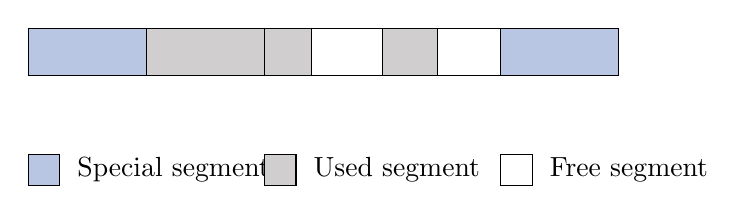
\begin{tikzpicture}
    \definecolor{specialsegment}{RGB}{184, 198, 228} %
    \definecolor{usedsegment}{RGB}{208, 206, 206}   %
    \definecolor{freesegment}{rgb}{1, 1, 1}            %

    \draw[fill=specialsegment, draw=black] (0, 0) rectangle (1.5, 0.6);  %
    \draw[fill=usedsegment, draw=black] (1.5, 0) rectangle (3, 0.6);     %
    \draw[fill=freesegment, draw=black] (3, 0) rectangle (4.5, 0.6);     %
    \draw[fill=usedsegment, draw=black] (3.0, 0) rectangle (3.6, 0.6);   %
    \draw[fill=usedsegment, draw=black] (4.5, 0) rectangle (6, 0.6);     %
    \draw[fill=freesegment, draw=black] (5.2, 0) rectangle (6, 0.6);   %
    \draw[fill=specialsegment, draw=black] (6, 0) rectangle (7.5, 0.6);  %

    \draw[fill=specialsegment, draw=black] (0, -1) rectangle (0.4, -1.4);
    \node[anchor=west] at (0.5, -1.2) {Special segment};

    \draw[fill=usedsegment, draw=black] (3, -1) rectangle (3.4, -1.4);
    \node[anchor=west] at (3.5, -1.2) {Used segment};

    \draw[fill=freesegment, draw=black] (6, -1) rectangle (6.4, -1.4);
    \node[anchor=west] at (6.5, -1.2) {Free segment};
\end{tikzpicture}
